\section{Описание разрабатываемой автоматизированной системы коммерческого учета энергоресурсов}

Автоматизированная система коммерческого учета энергоресурсов (АСКУЭ) - это программно-аппаратный комплекс, предназначенный для сбора, хранени и обработки инофрмации о потреблении энергоресурсов на объекте. 

Аппаратная часть представлена устройствами учета(УУ), устройствами сбора и передачи данных(УСПД), а так же центральным сервером(ЦС).

Программная часть включает в себя прошивки УУ и УСПД, ПО для ЦС.

ПО ЦС предназначено для сбора показаний с точек учета энергоресурсов, а также архивирования, хранения, анализа и визуализации полученных данных, формирования отчетов. Под показаниями подразумеваются данные о потребляемой мощности электроэнергии потребителями однофазных и трехфазных сетей.

Областью применения ПО ЦС являются объекты жилого, коммерческого и производственного назначения.

ПО ЦС — это программный комплекс, который должен включать в себя сервер баз данных, сервер сбора данных(ССД), сервер приложений, web-сервер, АРМ оператора, АРМ администратора, АРМ клиента, АРМ сервисного инженера.

ПО ССД должно выполнять следующие функции:
\begin{itemize}
 \item взаимодействие с УСПД и счетчиками (опрос и сбор данных);
 \item взаимодействие с СБД (запись обработанных данных для дальнейшей работы с ними);
 \item преобразование полученных данных в удобный для дальнейшей обработки формат;
 \item мониторинг и обработка ошибок;
 \item журналирование событий ССД.
\end{itemize}

ПО ЦС представляет собой иерархическую систему сбора, передачи и хранения данных (рис. \ref{irsh:irsh}). Информация от первичных приборов учета посредством УСПД поступает на ССД, который обеспечивает ее обработку и запись на СБД.

\begin{figure}[h!]
 \center{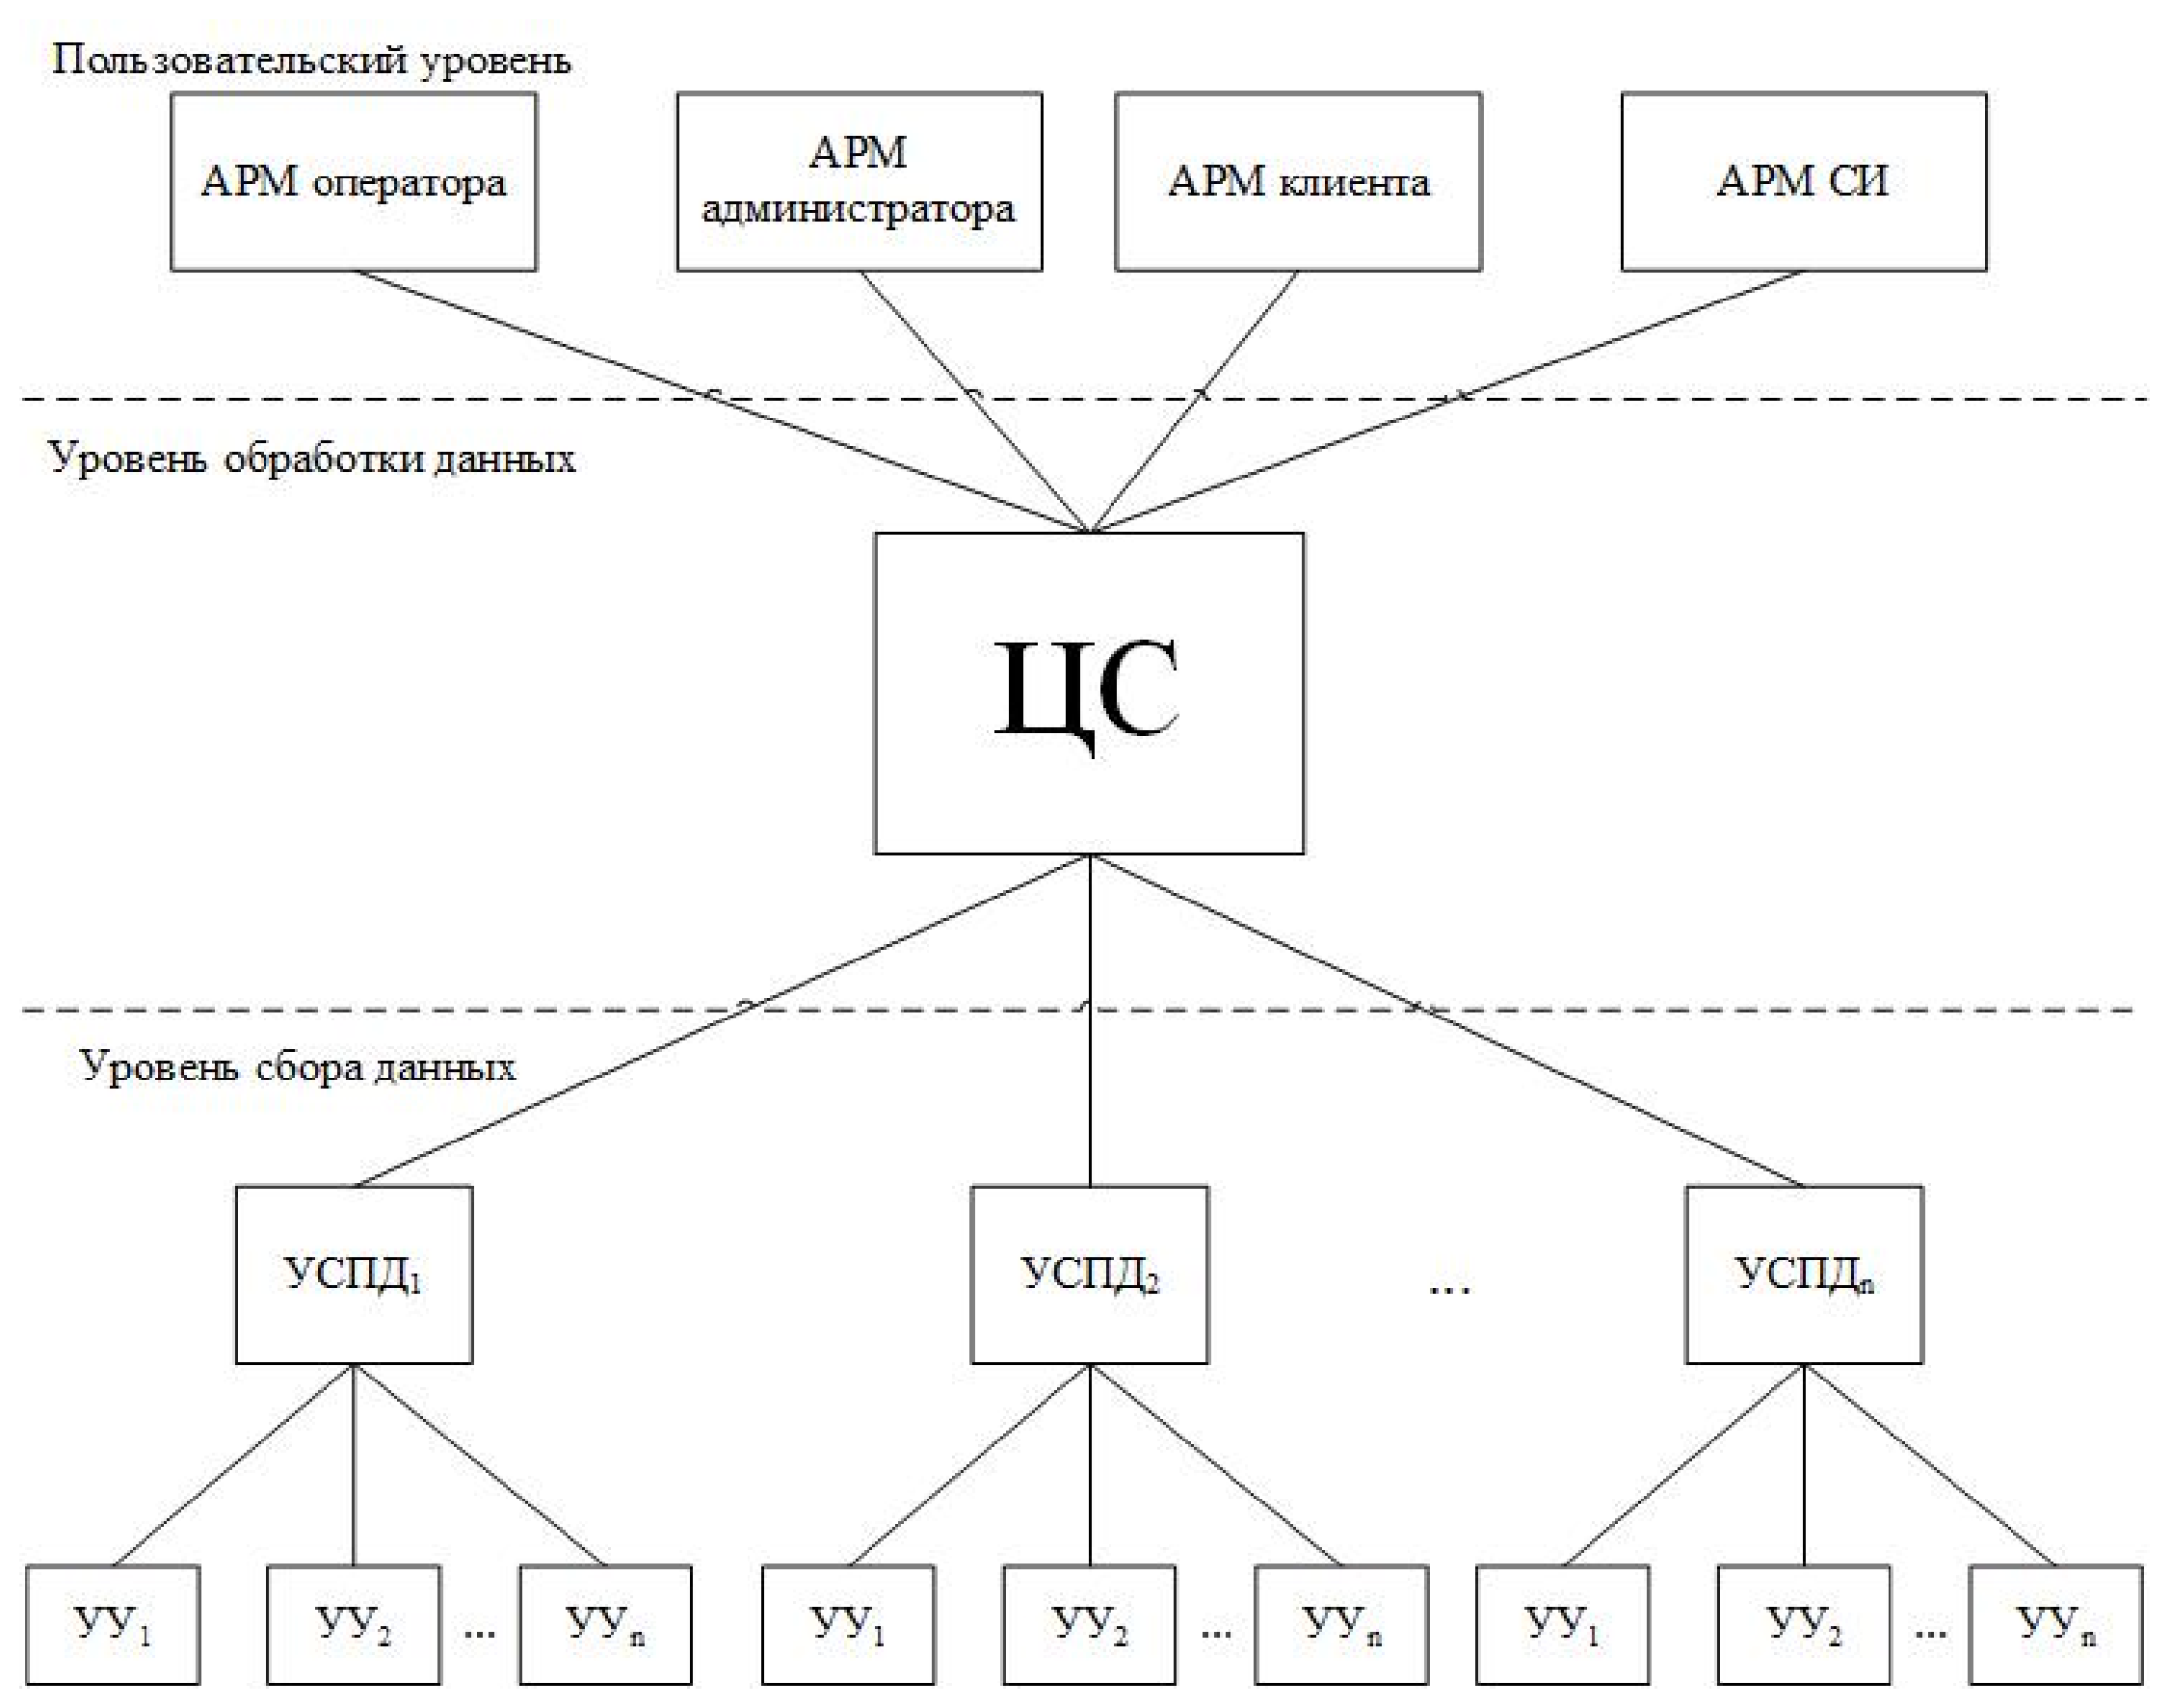
\includegraphics[width=0.8\linewidth]{irsh}}
 \caption{Структурная схема АСКУЭ}
 \label{irsh:irsh}
\end{figure}
